\documentclass[11pt,a4paper]{article}

\usepackage[utf8]{inputenc}
\usepackage[T1]{fontenc}
\usepackage[english]{babel}
\usepackage[a4paper,margin=2.4cm]{geometry}

\usepackage{amsmath, amssymb, amsthm}
\usepackage{mathtools}
\usepackage{booktabs}
\usepackage{tabularx}
\usepackage{array}
\usepackage{caption}
\usepackage{float}
\usepackage{enumitem}
\usepackage{microtype}
\usepackage{xcolor}
\usepackage{listings}
\usepackage{fancyhdr}
\usepackage{titlesec}
\usepackage{graphicx}
\usepackage{tikz}
\usetikzlibrary{positioning, arrows.meta, fit, backgrounds, calc, shapes.geometric}
\usepackage[hidelinks]{hyperref}

%  ---  Palette shared with the companion reports  ---
\definecolor{ink}{RGB}{26,30,36}
\definecolor{slate}{RGB}{92,101,112}
\definecolor{mist}{RGB}{233,235,238}
\definecolor{rulegrey}{RGB}{188,194,201}
\definecolor{steel}{RGB}{47,72,102}
\definecolor{steellight}{RGB}{124,146,172}
\definecolor{signal}{RGB}{160,32,45}

\hypersetup{
    colorlinks=true,
    linkcolor=steel,
    citecolor=steel,
    urlcolor=steel,
    pdftitle={A Link That Actually Falls: Communication Loss as an Event Rather Than a Declaration},
    pdfauthor={Haniel Ulises},
}

\color{ink}

\setlength{\headheight}{22pt}
\pagestyle{fancy}
\fancyhf{}
\fancyhead[L]{\small\textcolor{slate}{\itshape A Link That Actually Falls}}
\fancyhead[R]{\small\textcolor{slate}{\thepage}}
\renewcommand{\headrulewidth}{0.4pt}
\renewcommand{\headrule}{\hbox to\headwidth{\color{rulegrey}\leaders\hrule height \headrulewidth\hfill}}

\titleformat{\section}{\normalfont\large\bfseries\color{ink}}{\thesection}{0.7em}{}
\titleformat{\subsection}{\normalfont\normalsize\bfseries\color{ink}}{\thesubsection}{0.7em}{}
\titleformat{\paragraph}[runin]{\normalfont\bfseries\color{slate}}{}{0em}{}[.]

\captionsetup{font=small, labelfont={bf,color=slate}, textfont=footnotesize}

\theoremstyle{definition}
\newtheorem{definition}{Definition}
\newtheorem{proposition}{Proposition}
\newtheorem{remark}{Remark}

\lstdefinestyle{sys}{
    backgroundcolor=\color{mist},
    basicstyle=\ttfamily\scriptsize\color{ink},
    keywordstyle=\color{steel}\bfseries,
    commentstyle=\color{slate}\itshape,
    stringstyle=\color{slate},
    morecomment=[l]{\#},
    % Deliberately short. Most of the listings here are log excerpts, and
    % colouring their ordinary nouns marks a transcript as though it were
    % source. Only the declarations of the domain are highlighted.
    morekeywords={:types,:predicates,:objects,:agents,:goal,:init,site,agent},
    frame=single,
    rulecolor=\color{rulegrey},
    framesep=5pt,
    xleftmargin=6pt,
    xrightmargin=0pt,
    breaklines=true,
    showstringspaces=false,
    columns=fullflexible,
    captionpos=b,
}
\lstset{style=sys}

%  ---  Notation  ---
\newcommand{\Ag}{\mathcal{A}}
\newcommand{\Mod}{\mathcal{M}}
\newcommand{\Ev}{\mathcal{E}}
\newcommand{\prd}{\otimes}
\newcommand{\Kop}[1]{K_{#1}}
\newcommand{\Kw}[1]{\mathit{Kw}_{#1}}
\newcommand{\code}[1]{\texttt{\small #1}}
\newcommand{\site}[1]{\code{#1}}

\begin{document}

\begin{titlepage}
\centering
\vspace*{2.4cm}
{\color{rulegrey}\rule{\textwidth}{0.8pt}}\\[0.9cm]
{\LARGE\bfseries A Link That Actually Falls\par}
\vspace{0.5cm}
{\large\color{slate} Communication Loss as an Event Rather Than a Declaration,\\ and What a Map Is Once Two Robots Stop Agreeing\par}
\vspace{0.7cm}
{\color{rulegrey}\rule{\textwidth}{0.8pt}}\\[1.4cm]

{\large Haniel Ulises\par}
\vspace{0.3cm}
{\color{slate} Epistemic Robotics}\\
\vspace{0.15cm}
{\color{slate}\today}

\vfill
{\color{slate}\small
Every fleet in this series models restricted connectivity the same way. An
agent is oblivious to an announcement because the domain declares it oblivious;
the declaration is written before the run and no link ever falls. This report
cuts the radio between two robots during a run and measures what the declared
version cannot express.

\vspace{0.6em}
The apparatus is small and two findings from building it are not. The
announcement channel does not carry belief: it is read by a transcript recorder
and by nothing else, and the epistemic model advances through a service the
executor calls when an action completes, so a fault injector placed on the
channel measures nothing at all. And the reconciliation of two occupancy maps,
which passes forty-three tests over grids built in memory, refused the first
pair that two robots actually built, because a test that builds both grids
builds them the same shape and two maps that grow independently never are.

\vspace{0.6em}
A third finding is about measurement and not about the system. The first
version of the patrol driving the partner ran open loop and drove into the
racking, and a partner held against a rack does not move, so the propagated
belief tracked it perfectly. Correcting the collision raised the worst
estimation error by a factor of four. The defect was flattering the result.}
\vspace{1.2cm}
\end{titlepage}

\tableofcontents
\newpage

%  ======================================================================
\section{Scope}
\label{sec:scope}

A fleet in this series coordinates by speech. One robot senses, tells another
what it found, and a third is excluded; the domain declares who observes what,
the planner reasons over those declarations, and the executor dispatches the
actions they license. Restricted connectivity appears in that account exactly
once, as a property of an action type: an agent is \emph{oblivious} to an
event, which is a statement about a column of a relation and not about a radio.

The declaration is made before the run. It cannot be false during one, it
cannot be repaired, and nothing in the system can notice that the world stopped
matching it. This report removes that by cutting the link between two robots
while they work, and by measuring two things the declaration has no way to
express: what one robot's estimate of the other is worth while nothing arrives
from it, and what the two maps they built apart are worth once put together.

Three claims are established and are stated narrowly.

\begin{enumerate}[itemsep=3pt, topsep=4pt]
  \item An outage can be injected into a running fleet without modifying the
        fleet, and the cut is real in the only sense that matters, which is
        that the messages are counted as they are discarded.
  \item The belief propagation the requirement specifies exists, grows its
        covariance without decreasing it, and reaches the threshold past which
        it declares its own estimate unfit. Its acceptance criterion is met
        over outages of thirty, sixty and a hundred and twenty seconds against
        a partner in motion.
  \item The reconciliation of two occupancy maps runs on maps two robots built
        from two lasers in a simulator, which required one operation the layer
        did not have and which its unit tests could not have provoked.
\end{enumerate}

What is not established is set out in Section~\ref{sec:notestablished}, and one
item there is structural and not incidental: the epistemic models do not
diverge under partition, because there is one model for the fleet and not
one per robot, and a column of a shared relation is not a perspective held on
a vehicle.

%  ======================================================================
\section{What existed before}
\label{sec:before}

The requirement names two topics and an engine. The first thing the work
required was to find out what of that was code, and the answer determined the
design.

\begin{table}[H]
\centering\small
\caption{Occurrences of the artefacts the requirement names, across the three
repositories, excluding build trees. The count is of appearances in source, not
of definitions.}
\label{tab:inventory}
\begin{tabular}{@{}lrrl@{}}
\toprule
\textbf{Term} & \textbf{\code{eplansys}} & \textbf{\code{eplansys-rmf}} &
\textbf{This repository} \\
\midrule
\code{comm\_monitor}       & 0 & 0 & 0 \\
\code{BeliefUpdateEngine}  & 0 & 0 & 0 \\
\code{link\_down}          & 0 & 0 & 1, a string literal in a test \\
\code{link\_up}            & 0 & 0 & 7, an atom of a Kripke model \\
\bottomrule
\end{tabular}
\end{table}

The last row carries the whole difficulty. \code{link\_up} appears in the
warehouse scenario's model snapshots as
\code{labels: \{"w0": ["link\_up"]\}}: a proposition that a world makes true,
fixed when the problem was written, and a conjunct of a safety constraint
elsewhere. What existed of connectivity was the static declaration, and the
requirement was specification without implementation.

\subsection{The announcement channel does not carry belief}
\label{sec:channel}

The obvious injector subscribes to the channel two robots speak on and stops
forwarding. It would have measured nothing, and the reason is worth setting out
because it is a property of the architecture and not an accident of this
scenario.

The bridge publishes each speech act on
\code{/eplansys/channel/private/<listener>}. The only subscriber is the
transcript recorder, which exists so that who was addressed is a matter of
record and not of inference. The planner package contains no reference to
that channel. The model advances through a service,
\code{epistemic\_state/apply\_action}, which the executor calls when an action
completes, and in the performer for a speech act the two statements are
\code{speak()} and \code{conclude(true, \ldots)}, in that order.

\begin{proposition}[Gating the channel is epistemically inert]
\label{prop:inert}
Let $G$ be a filter that discards every message on the announcement channel
during $[t_{d}, t_{r}]$. Then for every action the policy dispatches in that
interval, the sequence of product updates applied to the epistemic state is the
same with $G$ as without it.
\end{proposition}

\begin{proof}
The state is advanced only by \code{apply\_action}, which the executor calls on
completion of an action. Completion is reported by the performer, which calls
\code{conclude} unconditionally after \code{speak}. Neither call reads the
channel, and no subscriber of the channel calls \code{apply\_action}. Hence the
argument to every \code{apply\_action} call, and the order of the calls, are
independent of $G$.
\end{proof}

The channel is an audit path. That is a reasonable thing for it to be, and it
is worth knowing before an experiment is built on the assumption that it is a
transport. The cut has to be placed where belief actually travels, which in
this system is the pose one robot receives from another and the map it is
handed.

\subsection{There is one epistemic model for the fleet}
\label{sec:onemodel}

The bringup runs one planner and one epistemic state. An agent's accessibility
relation is therefore a column of a shared structure and not a perspective held
on a robot, and two robots that stop communicating do not thereby acquire two
models to disagree with each other.

This bounds the report. What is measured here is the metric part of the
requirement, an estimate of a partner's pose and its covariance, and the
reconciliation of two maps. The divergence of modal structures is not measured,
because there are not two structures to diverge.

%  ======================================================================
\section{The apparatus}
\label{sec:apparatus}

Five components, in a package of their own. The fleet, the world and the
per-robot mapping are those of the companion report and are included unchanged.

\begin{table}[H]
\centering\small
\caption{The nodes of the scenario. Only the first three are required by the
requirement; the fourth exists because of what the first real pair of maps
did, and the fifth because the fleet's own driving does not work in this
workspace.}
\label{tab:nodes}
\begin{tabularx}{\textwidth}{@{}lX@{}}
\toprule
\textbf{Node} & \textbf{What it does} \\
\midrule
\code{comm\_monitor} &
Owns the state of the link and is the only thing that does. Publishes
\code{link\_down} and \code{link\_up}, latched, at the configured instants, and
answers a service for the state now. \\
\addlinespace
\code{link\_gate} &
The injector. A type-erased relay over the generic publisher and subscription,
so that one node cuts an odometry and an occupancy grid without a case for
either. It holds no timer and subscribes to the monitor like everything else. \\
\addlinespace
\code{belief\_update} &
The propagation. Holds the last received pose while the link is up; integrates
the last received twist forward while it is down, growing the covariance. Reads
the \emph{gated} odometry. \\
\addlinespace
\code{grid\_align} &
Places two maps on the union of their extents at their common resolution, by
whole-cell translation. \\
\addlinespace
\code{patrol} &
Drives the partner, because the measurement needs a partner in motion and the
fleet's own navigation cannot plan here. \\
\bottomrule
\end{tabularx}
\end{table}

Two decisions in the construction are load-bearing.

\paragraph{The gate is installed alongside, not in the middle} It reads the
topic the fleet already publishes and writes a second name that only the
believing side subscribes to. Nothing that exists is remapped, rebuilt or told
that a gate is present. Interposing properly, by renaming the producer's output
and taking over its name, also works and is what would be required to cut a
topic that existing nodes already read; it is not required here and would mean
editing a launch file four other demonstrations share.

\paragraph{The schedule is open loop} The link falls at $t_{d}$ and returns at
$t_{r}$, both measured from the monitor's first clock tick, and neither depends
on where the robots are. An outage triggered by separation would make its own
duration a function of the trajectory it perturbs, and the measurement could
not then separate the two.

\begin{remark}[The count is the evidence]
\label{rem:count}
The gate counts what it discards and reports the count when the link is
restored. A gate reporting zero discarded messages was gating a topic nobody
publishes on, which is a launch error that otherwise resembles a successful run
exactly. The propagation makes the symmetric check: it refuses a partner pose
that arrives while it believes the link is down, and says so, because an
arrival at that moment means the gate is on a different topic from the one
being read.
\end{remark}

\subsection{The partner has to move, and has to not crash}
\label{sec:patrol}

The requirement is a claim about a belief held while a partner is moving and
nothing is arriving from it. Measuring it needs the partner to move; it does
not need the partner to be pursuing the mission, and a trajectory that repeats
between runs is a better subject than one a planner improvises.

The first version drove a fixed square open loop and drove into the racking. A
warehouse is not empty, and open loop on a floor with shelving on it is a
collision with a timer attached. The square is now the intent and the laser is
the veto: below the clearance in the forward arc the robot turns instead of
advancing and keeps turning until the way is clear, with hysteresis on the way
out so that a robot clearing an obstacle by a millimetre does not advance, block
on the next scan, and shuffle along the face of the rack it is leaving.

\begin{remark}[The collision was flattering the measurement]
\label{rem:flattering}
This is the finding of the three, and it is a finding about measurement rather
than about the system. A partner held against a rack does not move. The
propagation integrates the last twist forward, so a stationary partner is
tracked perfectly and the estimation error stays near zero for reasons that
have nothing to do with the propagation. Correcting the collision raised the
worst error of the sixty-second outage from $1.774$ to $7.632$\,m. The run
looks worse and is worth more: the defect was producing agreement between the
belief and the partner by stopping the partner.
\end{remark}

%  ======================================================================
\section{The criterion, measured}
\label{sec:measured}

Three runs differing only in how long the link stays down. The partner drives
its patrol throughout and knows nothing of the outage. The bound is the
requirement's,
\[
  \varepsilon(\Delta t) \;=\; v_{\max}\,\Delta t \;+\; \sigma_{\mathrm{prop}},
  \qquad v_{\max} = 0.22\ \mathrm{m/s}, \qquad
  \sigma_{\mathrm{prop}} = 0.05\ \mathrm{m},
\]
with $v_{\max}$ taken from the maximum speed the fleet's own controller
enforces. Taking it from anywhere else would be measuring against a speed the
platform cannot reach.

\begin{table}[H]
\centering\small
\caption{The three runs. \emph{Margin} is the smallest difference between the
bound and the error over the outage, and \emph{trace} the positional covariance
when the link returned. Every figure is read from the record the run wrote.}
\label{tab:runs}
\begin{tabular}{@{}rrrrrrr@{}}
\toprule
\textbf{Outage} & \textbf{Samples} & \textbf{Worst error} & \textbf{At} &
\textbf{Margin} & \textbf{Breaches} & \textbf{Final trace} \\
\midrule
 30.0\,s &    325 &  3.634\,m &  30.0\,s & 0.040\,m & 0 & 0.600\,m$^2$ \\
 60.0\,s &    632 &  6.967\,m &  60.0\,s & 0.050\,m & 0 & 1.200\,m$^2$ \\
119.9\,s & 1\,247 & 19.199\,m & 119.9\,s & 0.040\,m & 0 & 2.398\,m$^2$ \\
\bottomrule
\end{tabular}
\end{table}

The criterion is met in all three. The covariance behaves as specified: the
trace grows without decreasing and crosses $\sigma_{\max}^2 = 1.0$\,m$^2$ at
fifty seconds, at which point the engine reports that where the partner is
should no longer be believed.

Two features of the table are worth more than the verdict.

\paragraph{The worst error is at the end, and grows with the outage} It was not,
before the patrol was corrected. A partner intermittently held against a rack
produced a worst error of $1.774$\,m at sixty seconds and a smaller one at a
hundred and twenty than at sixty, which is the signature of a measurement whose
subject was not moving. With the collision removed the three worst errors are
monotone in the duration and each occurs at the last sample.

\paragraph{The margin is tightest at the start} In all three runs the smallest
difference between the bound and the error is at $\Delta t = 0$, where the
bound is $\sigma_{\mathrm{prop}}$ alone and the error is a few millimetres of
odometry noise. It is not tightest at the end, where the error is largest.

\subsection{The bound is loosest where the estimate is worst}
\label{sec:loose}

The second observation is a property of the criterion and not of this
implementation, and it is worth stating precisely because a passing verdict
invites the opposite conclusion.

\begin{proposition}[The criterion cannot fail against a partner that holds its course]
\label{prop:course}
Let the partner be a differential-drive body that keeps the pair
$(v, \omega)$ it had at $t_{d}$, and let the propagation integrate that same
pair from the same pose. Then the estimation error is identically zero and the
criterion is satisfied for every $\Delta t$. If instead the partner reverses at
full speed at $t_{d}$, the error is $2 v_{\max} \Delta t$ and the criterion
fails for every $\Delta t > \sigma_{\mathrm{prop}} / v_{\max}$.
\end{proposition}

\begin{proof}
For the first part, both integrations start from the same pose with the same
twist and are the same function of time, so their difference vanishes and lies
below any positive bound. For the second, the belief advances $v_{\max}\Delta t$
along the original heading and the partner the same distance against it, so the
separation is $2 v_{\max}\Delta t$. Requiring
$2 v_{\max}\Delta t > v_{\max}\Delta t + \sigma_{\mathrm{prop}}$ reduces to
$v_{\max}\Delta t > \sigma_{\mathrm{prop}}$.
\end{proof}

With the values used here the threshold of Proposition~\ref{prop:course} is
$0.23$\,s. The bound is therefore broken within the first quarter second of the
outage for the worst case it admits, and cannot be broken at all for the best.
The measured runs sit between the two: the patrol holds its course along the
straight legs, which are most of the path, and turns at the ends, and the error
that accumulates is the turning. At a hundred and twenty seconds it reaches
$19.2$\,m against a bound of $26.5$\,m, which is the closest any of the three
comes.

What the runs establish is that the propagation tracks a partner behaving as
this one behaves. They do not establish that the bound is a useful guarantee,
and Proposition~\ref{prop:course} says it is not one in the case it was
presumably written for.

%  ======================================================================
\section{Reconciliation on maps two robots built}
\label{sec:reconciliation}

The collaborative layer classifies cells against thresholds, computes per-robot
coverage, detects contradictions and reconciles. It passes forty-three tests.
Every one of them builds both grids in memory, and a test that builds both
grids builds them the same shape.

Two maps that two robots actually built are never the same shape. Each grows as
its own robot discovers floor, and the first pair this reconciliation was ever
handed came back \code{grids differ in size: 118x128 and 134x86}.

\begin{remark}[A refusal its own tests could not provoke]
\label{rem:refusal}
The refusal is correct and is not weakened here. Two maps whose discretisation
does not coincide are declined and not approximated, because a wrong
registration produces a merged map that is confidently wrong, which is worse
than one that is obviously incomplete. What is worth recording is that the
refusal path had never executed: the suite covered the fusion and not its
negative, and not through carelessness. The bench cannot produce the situation
that provokes it, because the situation is two independent map processes and
the bench has none.
\end{remark}

The missing operation is placement, not registration. Both maps come from the
same simulator at the same resolution, so putting them on a common extent is a
translation by whole cells: no interpolation, no rotation, no scaling, and a
cell keeps the value it had. Maps at differing resolutions are still refused,
because putting those on one grid would be the approximation the layer declines
to make.

\begin{figure}[H]
\centering
\begin{tikzpicture}[x=1mm, y=1mm, font=\scriptsize]
  \tikzset{
    grid/.style={draw=slate, line width=0.5pt},
    seen/.style={fill=mist},
    union/.style={draw=signal, line width=0.7pt, dash pattern=on 1.6pt off 1.4pt},
    lbl/.style={font=\scriptsize, text=slate, align=center}}

  % --- the two maps as their own extents
  \fill[seen] (0,0) rectangle (26,28);
  \draw[grid] (0,0) rectangle (26,28);
  \node[lbl] at (13,-4) {r2's map\\$117 \times 128$};

  \fill[seen] (40,6) rectangle (70,25);
  \draw[grid] (40,6) rectangle (70,25);
  \node[lbl] at (55,-4) {r1's map\\$133 \times 86$};

  % --- the union
  \begin{scope}[xshift=88mm]
    \fill[seen] (0,0) rectangle (26,28);
    \fill[seen] (18,6) rectangle (48,25);
    \draw[grid] (0,0) rectangle (26,28);
    \draw[grid] (18,6) rectangle (48,25);
    \draw[union] (0,0) rectangle (48,28);
    \node[lbl] at (24,-4) {the union they are placed on\\$134 \times 397$ at $0.050$\,m per cell};
  \end{scope}

  \draw[-{Latex[length=1.8mm]}, slate] (74,14) -- (84,14);

  \node[lbl, anchor=north west, text width=136mm] at (0,-12)
    {Extents, not contents. The overlap is where the two robots both have an
     opinion and is where a contradiction could arise; in the runs reported
     here it is empty of disputes, because the believing robot holds its dock
     and the partner patrols elsewhere. The union grows as both maps grow, so
     the figure is of one instant and the cell counts of
     Table~\ref{tab:fusion} are of the instant the link returned.};
\end{tikzpicture}
\caption{What \code{grid\_align} does. It is a whole-cell translation onto the
union of the two extents, and it exists because the layer refuses a pair it
cannot place, which is the right refusal and had never been reached.}
\label{fig:align}
\end{figure}

\begin{table}[H]
\centering\small
\caption{What the fusion reported at reconnection. The counts are the
fusion's own, from its reply, and are not a recount: an earlier version of the
recorder differenced cell counts it had subscribed to itself and reported a
merged map with fewer decided cells than one of its inputs, because the aligner
keeps publishing as both maps grow and the pair in hand when a reply arrives
need not be the pair the fusion was given.}
\label{tab:fusion}
\begin{tabular}{@{}rrrrr@{}}
\toprule
\textbf{Outage} & \textbf{Cells} & \textbf{Believer learns} &
\textbf{Partner learns} & \textbf{In conflict} \\
\midrule
 30.0\,s & 65\,505 & 5\,537 & 4\,917 & 0 \\
 60.0\,s & 65\,505 & 5\,556 & 4\,872 & 0 \\
119.9\,s & 65\,505 & 4\,879 & 4\,903 & 0 \\
\bottomrule
\end{tabular}
\end{table}

Each robot learns from the other close to the count the other had decided, and
nothing is in conflict. That is not the reconciliation being clever; it is what
a disjoint pair of observations looks like. The believing robot holds its dock
and maps what it can see from there, the partner patrols elsewhere, and the two
sets of observed cells barely meet. A conflict requires two robots to have
observed one cell and disagreed about whether it is passable, and this pair
never did.

The zeros are therefore a property of the trajectory and not a result about the
fusion. Producing a genuine contradiction requires routing the two through one
aisle from opposite ends, which is the next run and not this one.

%  ======================================================================
\section{Defects}
\label{sec:defects}

Three, and the third is the one worth carrying.

\begin{table}[H]
\centering\small
\caption{What was found by running the integration, and how each presented.}
\label{tab:defects}
\begin{tabularx}{\textwidth}{@{}p{0.26\textwidth}X@{}}
\toprule
\textbf{Defect} & \textbf{Presentation} \\
\midrule
Stale binary interface &
Every action node died at startup with \code{undefined symbol:
ActionExecutorClient::finish(bool, float, string const\&)}. The installed
binaries were built when \code{finish} took three arguments; it now takes four,
the fourth being the outcome the epistemic extension needs. A rebuild fixes it,
and nothing warns that an installed tree is older than the library it links. \\
\addlinespace
The fleet cannot drive with two robots &
One robot's global costmap never receives its map, keeps the default five-metre
extent at the origin, reports the robot out of bounds, and the navigation
cannot plan. The topic exists with one publisher and five subscribers and the
costmap's own parameter names it. Not diagnosed further; the scenario drives
the partner directly instead. \\
\addlinespace
The patrol drove into the racking &
An open-loop square on a floor with shelving on it. The consequence was not a
crashed run but a flattering one: a partner held against a rack does not move,
and a propagation that integrates the last twist tracks a stationary partner
exactly. See Remark~\ref{rem:flattering}. \\
\bottomrule
\end{tabularx}
\end{table}

The third is a defect in the instrument and not in the system under test,
and it is the kind this series keeps finding: not a component that fails, but
an arrangement in which every component behaves correctly and the number that
comes out measures something other than what was intended. The gate discarded
its messages, the propagation integrated its twist, the recorder compared
against the ungated truth, and the answer was still wrong, because the subject
of the measurement had stopped moving for a reason nobody had asked about.

%  ======================================================================
\section{What the runs establish}
\label{sec:established}

That an outage can be injected into a running fleet without modifying it, and
that the cut is real and counted: 1\,764 odometry messages and 64 map messages
discarded in the sixty-second run, against 1\,179 and 41 that passed before it.

That the propagation exists, grows its covariance monotonically, and reaches
the threshold past which it declares its own estimate unfit to be believed.

That its acceptance criterion is met over outages of thirty, sixty and a
hundred and twenty seconds against a partner in motion, with the qualification
of Proposition~\ref{prop:course} attached.

And that the reconciliation runs on maps two robots built from two lasers in a
simulator, which required an operation the layer did not have and which its own
tests could not have provoked.

\section{What they do not}
\label{sec:notestablished}

They do not establish that the epistemic models diverge under partition,
because there is one model for the fleet. Two robots that stop communicating do
not thereby acquire two structures to disagree with each other, and an
accessibility relation here is a column of a shared structure and not a
perspective held on a vehicle. Section~\ref{sec:onemodel} states this and
Section~\ref{sec:next} says what it would take to remove it.

They do not establish that the fused state satisfies the goal at reconnection
by the validator's account, for the same reason. There is one model, it never
diverged, and a check against it would be a check that nothing was partitioned.

They do not establish anything in favour of the bound.

And they do not establish that the fusion resolves contradictions well, because
it was never given one.

%  ======================================================================
\section{What would remove the limitation}
\label{sec:next}

The obstacle is one shared model, and the path to two is shorter than it looks.
Three properties of the existing code decide it, and all three were checked
and not assumed.

\begin{enumerate}[itemsep=4pt, topsep=4pt]
  \item \textbf{The state node namespaces cleanly.} Every service and topic
        name in it is relative; the package contains no absolute name. Launching
        it under \code{r1} and again under \code{r2} yields
        \code{/r1/epistemic\_state/apply\_action} and its counterpart, two
        independent models, with no change to the planner.
  \item \textbf{A reconciliation primitive already exists.}
        \code{epistemic\_state/announce} takes a formula, keeps the worlds where
        it holds, and increments a belief version precisely because the
        information arrived outside the plan. Replaying into a model what it
        missed is one call per missed finding.
  \item \textbf{The gate already cuts where it would need to.} It gates by
        topic and type; the path carrying an update to an absent agent's model
        is one more entry in a launch file.
\end{enumerate}

What would have to be written is a router: today the executor calls one model,
and it would have to call each, applying the observability rule the domain
declares. That is new code in the scenario package, not a modification of the
planner.

One caveat belongs with the proposal. \code{announce} implements a public
announcement, so replaying a missed private one makes its content common
knowledge in the model that missed it. Reconciliation by replay therefore
returns a model that is \emph{compatible} with the one that never lost the
link, and not identical to it. That is the right target and not a
shortcoming: what reconciliation should restore between two structures that
observed different things is their compatibility, and requiring equality would
falsify one of them to preserve a consistency the domain does not demand.

%  ======================================================================
\section*{Reproduction}
\addcontentsline{toc}{section}{Reproduction}

\begin{lstlisting}
colcon build --packages-select epistemic_msgs epistemic_comm epistemic_slam
colcon test --packages-select epistemic_comm          # 62 tests

ros2 launch epistemic_comm link_outage_launch.py \
     t_disc:=70 t_recon:=130 scenario:=baseline
\end{lstlisting}

\noindent
\code{t\_disc} and \code{t\_recon} are seconds from the monitor's first clock
tick. Two records are written per run, one of the belief error against the
bound at every sample and one of the reconciliation, and the figures in
Tables~\ref{tab:runs} and~\ref{tab:fusion} are read from them.

\end{document}
